
%Inicio del Preámbulo: Modifícalo bajo tu propio riesgo! Usa los paquetes que requieras para 
%implementar funcionalidades dentro del documento. Se comenta solo lo esencial, puedes buscar los
%paquetes y documentarte de su funcionalidad y puedes eliminarlos también si así lo deseas. 

\documentclass[letterpaper,12pt]{article} %Modifica el tipo de documento y el tamaño de la letra.
\usepackage[T1]{fontenc}
\usepackage{mathptmx}
\usepackage[utf8]{inputenc} %Formato UTF-8 para caracteres especiales.
\usepackage[shortlabels]{enumitem}
\usepackage[spanish,mexico]{babel} 
\usepackage{amsmath,amssymb,amsfonts,latexsym,cancel}
\usepackage{hyperref}
\usepackage{wrapfig}
\usepackage[rflt]{floatflt}
\usepackage[pdftex]{graphicx}
\usepackage{fancyhdr} %Paquete para el header y el formato de la portada. No sugiero borrarlo!
\usepackage{float}
\usepackage{longtable,multirow,booktabs}
\usepackage{cite}
\usepackage{wrapfig}
\usepackage[square,numbers]{natbib}
\usepackage{multicol}
\usepackage{caption}
\usepackage[]{sidecap}
\usepackage{adjustbox}
\usepackage{parskip}
\usepackage{enumitem}
\usepackage{tikz}
\usepackage{lipsum}
\usepackage[]{xcolor}
\usepackage{subcaption}
\graphicspath{Imágenes/}
\usepackage{listings}
\usepackage{color}
\usepackage{minted}

\definecolor{dkgreen}{rgb}{0,0.6,0}
\definecolor{gray}{rgb}{0.5,0.5,0.5}
\definecolor{mauve}{rgb}{0.58,0,0.82}

\lstset{frame=tb,
  language=HTML,
  aboveskip=3mm,
  belowskip=3mm,
  showstringspaces=false,
  columns=flexible,
  basicstyle={\small\ttfamily},
  numbers=none,
  numberstyle=\tiny\color{gray},
  keywordstyle=\color{blue},
  commentstyle=\color{dkgreen},
  stringstyle=\color{mauve},
  breaklines=true,
  breakatwhitespace=true,
  tabsize=3
}


%Fin de Préambulo


%Inicio formato de Página. Puedes establecer medidas de la página y modificar el header.

\textheight = 21cm %Medidas de la  página
\textwidth = 18cm  %Medidas de la página
\topmargin = -2cm  %Medidas de la página    
\oddsidemargin = -0.8cm %Medidas de la página
\pagestyle{fancy} %Diseño de la página


\fancyhf{}
\lhead{}%%LeftHead
\chead{
\includegraphics[width=1cm, height=1cm]{Imágenes/logo-itcj.jpg}}%%CenterHead
%\lfoot{USM}
\rhead{Taller de Sistemas Operativos}%%RightHead

\setlength{\columnsep}{4mm}%Comandos para el formato de la página.
%\setlength{\parindent}{4em}%Sangría al comenzar un nuevo párrafo.
\setlength{\parindent}{0.5in}
%\setlength{\parindent}{4em}%Sangría al comenzar un nuevo párrafo.
\setlength{\parskip}{1em}%Distancia entre párrafos.
\renewcommand{\baselinestretch}{1.5}% Espacio entre línea y línea o interlineado.
\setlength{\headheight}{33pt}
\fancyfoot[LE, RO]{\thepage} %Logo de LaTeX y pie de página.

%Fin formato de Página

%Aquí inicia el documento. Date como magnate
\begin{document}

    %LaTeX te hace el índice automáticamente conforme añades secciones en tu documento.
    \thispagestyle{empty}
			\begin{figure}[ht]
		   \minipage{\textwidth}
		        \centering
				
\includegraphics[width=3cm]{Imágenes/logo-itcj.jpg}
				\label{escudoTEC}
		   \endminipage
				%%\vspace{-1cm}
		\end{figure}
		
		\vspace{0.1cm}
		
		\begin{center}
		    {\scshape\LARGE \textbf{Instituto Tecnológico de Ciudad Juárez} \par}
            
             {\LARGE Ingeniería en Sistemas Computacionales \par}
             {\LARGE Taller de Sistemas Operativos}

			% Restauramos el interlineado:
			\begin{center}
			
			{\LARGE \textit{Grupo: C - Semestre: Enero-Junio 2022}}

			{\LARGE\bfseries Práctica Servidor Web.\par}

		{\scshape\Large Fecha: 06/03/2022\par}	

			        \LARGE	{ \textbf{Profesor:}}\\%% \textbf son negritas
        \large		{M.S.L Noé Ramón Rosales Morales}
        
		\vspace{-0.5cm}	
		
		\LARGE	{ \textbf{Alumno(s):}}\\%% \textbf son negritas

        \normalsize	 {Cardona Silveyra Juan Carlos - 20112050}
        
        \vspace{-0.5cm}
        
        \normalsize		{Hernandez Zermeño Esmeralda Guadalupe - 20112073}
        
        \vspace{-0.5cm}
        
        \normalsize		{García Rangel Gabriel Antonio - 20112079}
        
        \vspace{-0.5cm}
        
        \normalsize		{Gomes Perez Luis Arturo - 20112083}

        
        
%% \it es letra itálica
				\vspace{1.25cm}
				\vspace{0.9cm}
				
			\end{center}
	
		\end{center}
    \tableofcontents
    \newpage
    \listoffigures
%Inicio parte opcional. Esta parte la puedes quitar si deseas, es por si te piden formatos para
%evidencias de certificación de los laboratorios con números de cuenta o te piden abstracts en tus %trabajos.

\title{Taller de Sistemas Operativos \\\textbf{Práctica Servidor Web} \\ }
\date{}

\maketitle
\thispagestyle{fancy}

%Fin parte opcional

\section{Introducción}
Los servidores son una tecnología sumamente importante en la sociedad de hoy en día. En una economía global donde se ha creado la necesidad de continuas innovaciones tecnológicas para ventajas competitivas, los servidores ofrecen diversas características tales como una configuración centralizada, acceso a grandes cantidades de datos, entre otros que logran satisfacer dichas necesidad de competitividad.\cite{zapico2007new}\cite{servers}\par

El objetivo de esta práctica es mostrar la creación de un servidor web con el servicio IIS a través del sistema operativo de servidor Windows Server 2016 y como conectarse a este mismo a través de otra maquina. Con el fin de guiar al lector que este iniciando sus conocimientos en esta rama de la tecnología.

%\

\newpage
\vspace{1cm}

\section{Marco Teórico}

Para un mejor entendimiento de la presente práctica se necesitan tener los siguientes conocimientos previos:

\begin{itemize}
   \item \textbf{Servidor: } Maquina que provee distintas funcionalidades a otras maquinas llamadas "clientes", entre estas tareas esta la capacidad de compartir información, recursos del dispositivo y realizar tareas computacionales.

    \item \textbf{Sistema operativo de servidor: } Es un conjunto de programas que tienen la funcion de gestionar recursos de una computadora tanto hardware y software a la vez es una interface entre la maquina y el usuario, especificamente hecho para maquinas servidor.
    
    \item \textbf{Windows Server: } Plataforma para la construcción de la infraestructura de aplicaciones interconectadas y servicios web.\cite{MSServer} Básicamente un sistema operativo de servidor.
    
    \item \textbf{IP: }Internet Protocol, se refiere a una dirección especifica de una maquina en la red.\cite{comer2013internetworking}
    
    \item \textbf{DNS: } Domain Name Service, Sistema que asigna un nombre a una dirección en el internet.\cite{comer2013internetworking}
    
    
\end{itemize}



\section{Desarrollo de la Práctica}


\subsection{Instalación de IIS (Internet Information Server)}

IIS es el termino utilizado para un servidor web de proposito general que utiliza el sistema operativo Windows.
%Recordatorio de citar algo aqui%
El IIS acepta y responde las peticiones de maquinas cliente, además, de permitir compartir información a través de una red LAN. Sirve como host de aplicaciones, sitios web, entre otros para compartir con los usuarios. En esta sección de la práctica se mostrara la instalación de este servicio.

\begin{itemize}
    \item Para empezar, se debe abrir la aplicación de administrador de servidor donde permite configurarlo.
    \item Dirigirse a la opción de agregar roles y características y seleccionar la opción de \textbf{instalación basada en roles} como se muestra en la figura 1.
    
    \begin{figure}[htp!]
        \centering
        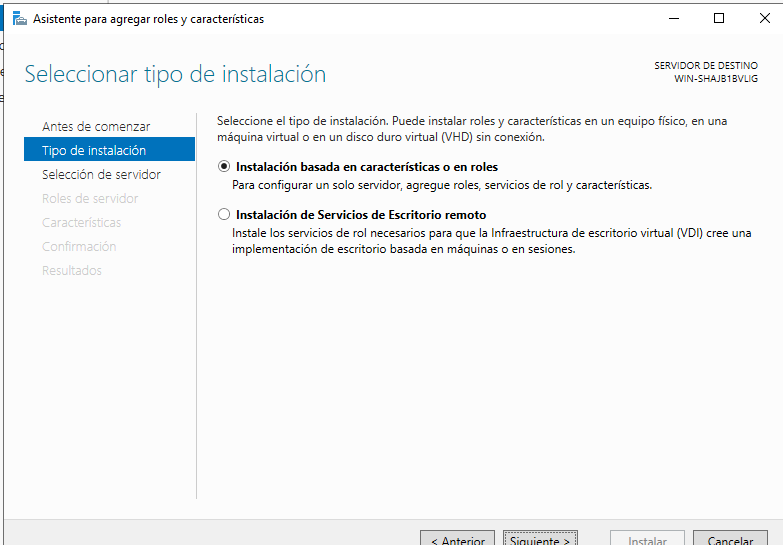
\includegraphics[width = 9cm, height = 9cm]{Imágenes/instalacion_roles_p2.jpg}
        \caption{Instalación basada en roles.}
        \label{fig:instalacion_roles}
    \end{figure}
    
    \newpage
    
    \item Posteriormente en la sección de Selección de Servidor, se selecciona la maquina que sera el servidor y en los roles se elegirá el servicio IIS (Figura 2).
    
    \begin{figure}[htp!]
        \centering
        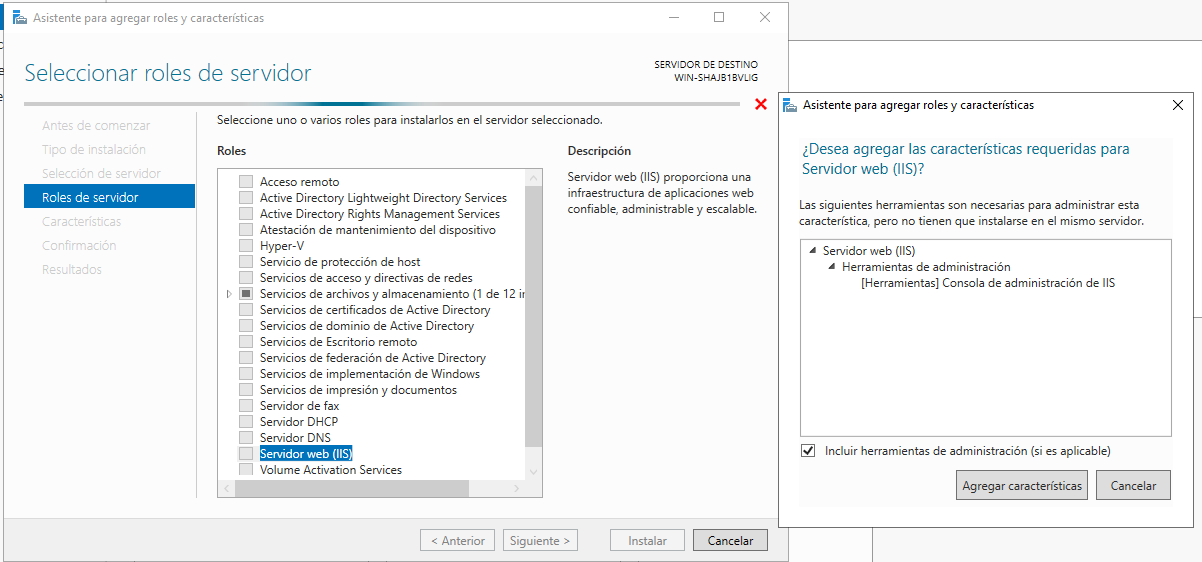
\includegraphics[width = 9cm, height = 9cm]{Imágenes/servicio_iis.jpg}
        \caption{Servidor Web (IIS)}
        \label{fig:servicio_iis}
    \end{figure}
    
    
    \item Para fines de la práctica y para prevención de errores, se activaron las siguientes características que se presentan para el servidor: Activación de canalizaciones por nombre, Message Queing, TCP, HTTP, Message Queue Server, Nucleo de web hospedable ISS. Después de estos pasos el servicio IIS estará finalmente instalado en la maquina servidor.
    
    \begin{figure}[htp!]
        \centering
        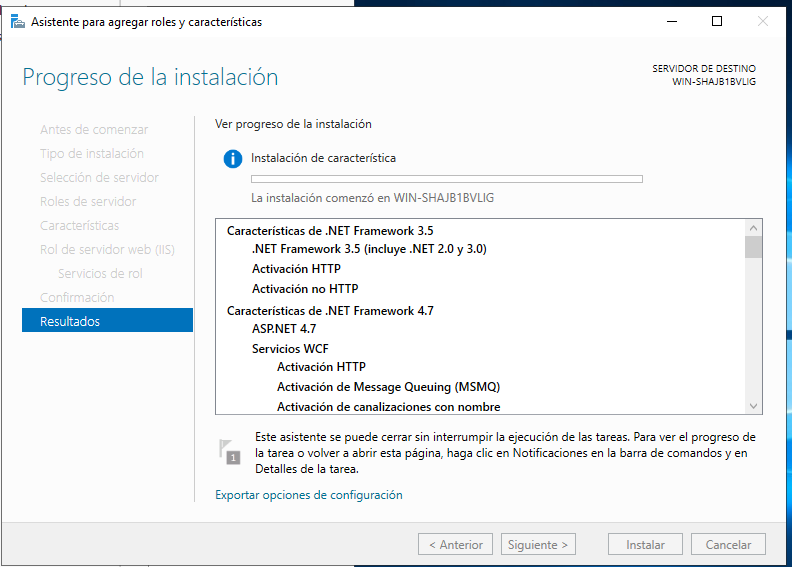
\includegraphics[width = 9cm, height = 9cm]{Imágenes/caracteristicas_servidor.jpg}
        \caption{Características del servidor.}
        \label{fig:caracteristicas_servidor}
    \end{figure}
\end{itemize}

\newpage

\subsubsection{Activación del IIS Actualizado}
Para activar el servicio IIS con las características que se especificaron, se debe iniciar como administrador el Windows PowerShell e introducir el siguiente comando:\par

\textit{Install-WindowsFeature -name Web-Server -IncludeManagmentTool}


\begin{figure}[htp!]
    \centering
    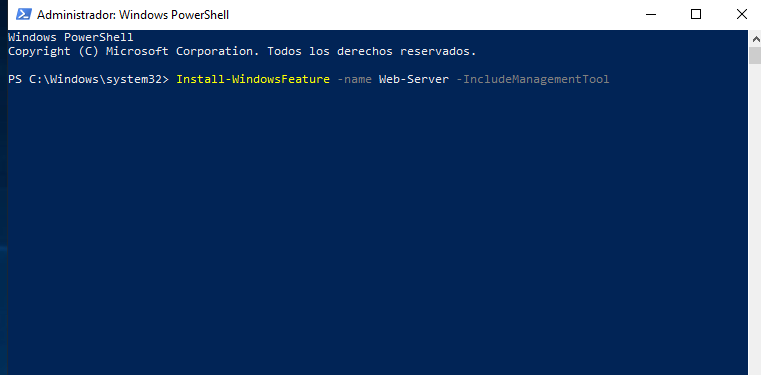
\includegraphics[width = 9cm, height = 9cm]{Imágenes/powershell_admin.jpg}
    \caption{Activación del servicio IIS}
    \label{fig:activacion_iis}
\end{figure}


\newpage

\subsection{Configuración del IP}
Para que otras maquinas puedan comunicarse al servidor, este requiere una dirección IP, la cual permite que la transmisión de datos entre maquinas tenga una dirección origen y destino. En esta sección de la práctica se observara como configurar la IP para un servidor y como se puede comprobar la conectividad entre maquinas a través del command prompt.

Para configurar la IP de la maquina servidor se debe hacer lo siguiente:

\begin{itemize}
    \item En el de panel de control dirigirse al apartado de centro de redes.
    \item Una vez en el centro de redes en el centro de redes, seleccionar las propiedades de la red que se dispone.
    \item En propiedades de la red, seleccionar la sección \textbf{Protocolo de Internet versión 4 (TCP/IPv4)}. 
    \item Al seleccionar el protocolo anteriormente mencionado, se mostrara un menú donde se podrá configurar la dirección IP de la maquina servidor (Figura 4). Para fines de la práctica se opto por utilizar la dirección 192.168.1.100 y un DNS con el mismo identificador. Una vez realizado estos pasos la configuración esta completada.
    
    \begin{figure}[htp!]
        \centering
        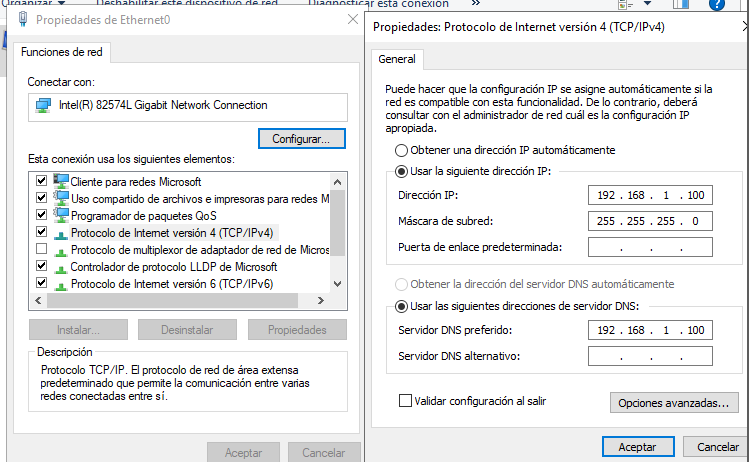
\includegraphics[width = 8cm, height = 8cm]{Imágenes/menu_ip.jpg}
        \caption{Configuración de dirección IP.}
        \label{fig:menu_ip}
    \end{figure}
    
\end{itemize}

Una vez completada la configuración de la IP se necesita comprobar si funciona la conectividad a la maquina servidor. Para eso se utilizara una maquina cliente donde ejecutaremos el siguiente comando en el command prompt:\par

\textit{ping <destino>}\par

En este caso se utilizara la dirección 192.168.1.100 como destino, ya que, es la dirección de la maquina servidor.

\begin{figure}[htp!]
    \centering
    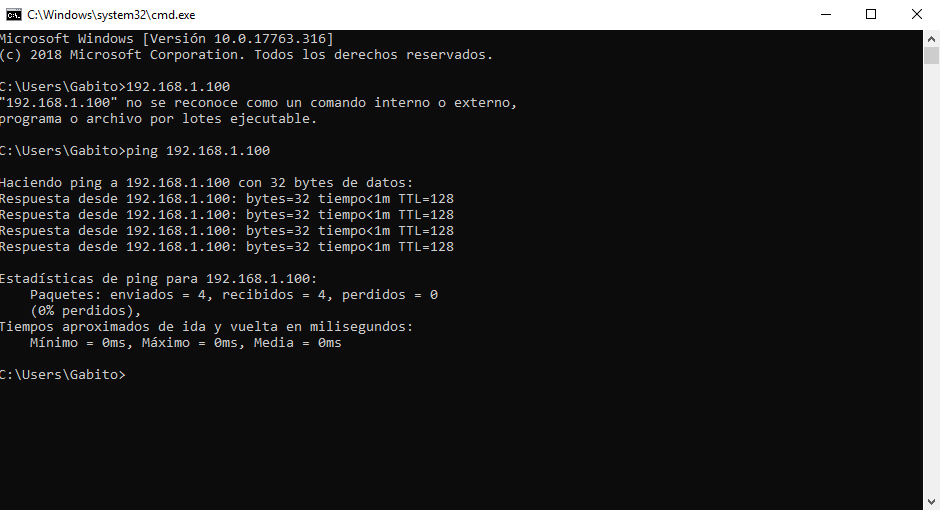
\includegraphics[width = 9cm, height = 9cm]{Imágenes/ping_ghc.jpg}
    \caption{Conectividad entre maquinas exitosa.}
    \label{fig:ping_ghc}
\end{figure}

\newpage

\subsection{Conectándose a una pagina web del servidor desde una maquina cliente.}

Una vez configurado el servicio IIS, la maquina esta preparada para ser un servidor web funcional. Para esta practica se utilizo un pequeño proyecto web para representar la compañía GHC.

Para empezar:
\begin{itemize}
    \item Abrir el administrador IIS en la maquina servidor.
    \item En configuraciones avanzadas seleccionar la opción de Administrar sitio web, configurar el adaptador y seleccionar la carpeta donde se encuentra el código del sitio web como se muestra en la figura 7.
    
    \begin{figure}[htp!]
        \centering
        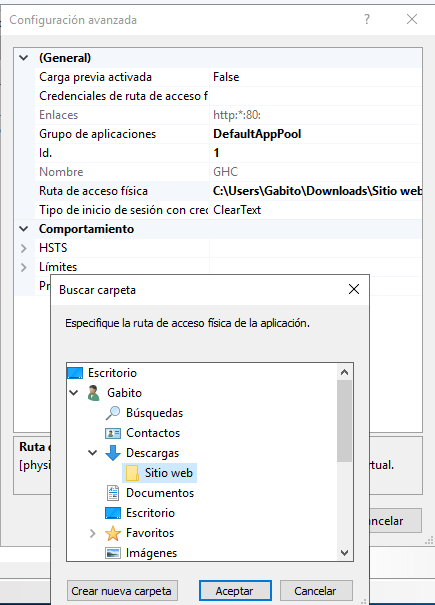
\includegraphics[width = 9cm, height = 9cm]{Imágenes/sitio_web.jpg}
        \caption{Selección del sitio web}
        \label{fig:sitio_web}
    \end{figure}
\end{itemize}

\newpage

Una vez seleccionado el sitio web, para probar la conectividad se accederá desde una maquina cliente a través de un navegador donde en la barra de búsqueda se buscara la IP del servidor web, la cual es 192.168.1.100. Una vez realizado lo anterior, se mostrará la página web de GHC.

\begin{figure}[htp!]
    \centering
    
\includegraphics[width = 9cm, height = 9cm]{Imágenes/ghc.jpg}
    \caption{Página web de GHC.}
    \label{fig:ghc}
\end{figure}

\newpage

\textbf{Código utilizado para la página web: }

\begin{lstlisting}
<!DOCTYPE html PUBLIC "-//W3C//DTD XHTML 1.0 Transitional//EN" "http://www.w3.org/TR/xhtml1/DTD/xhtml1-transitional.dtd">
<html xmlns="http://www.w3.org/1999/xhtml">
<head>
<meta http-equiv="Content-Type" content="text/html; charset=iso-8859-1" />
<title>GHC</title>
<style type="text/css">
<!--
.Estilo2 {font-size: 65px}
-->
</style>
</head> 
<link rel="stylesheet" type="text/css" href="estilos_ghc.css" />
<body>
<h1><center> 
  <span class="Estilo2">GHC </span>
</center></h1>
<h2> <center>Ciberseguridad </center></h2>
<center>
<div id="header">
<center>
			<ul class="nav">
				<li><a href="">Inicio</a></li>
				<li><a href="">Mision</a></li>
				<li><a href="">Vision</a></li>
				<li><a href="">Contacto</a></li>
			</ul>
			</center>
		</div>
		</center>
		<br />
		<div class="container">
  
  <ul class="slider">
    <li id="slide1">
      <img src="https://tec.mx/sites/default/files/styles/header_full/public/2021-08/ciberseguridad
      -tec
      -de-monterrey.jpg?itok=H3ibmb8t"/>    
      </li>
    <li id="slide2">
      <img src="https://d9b6rardqz97a.cloudfront.net/blog/wp-content/uploads/2020/07/28120744
      /Ciberseguridad-en-empresas-1080x567.jpg"/>    </li>
    <li id="slide3">
      <img src="https://revistabyte.es/wp-content/uploads/2020/03/teletrabajo
      -ibm-alerta-de-los-riesgos-de-ciberseguridad.jpg"/>    </li>
  </ul>
  
  <ul class="menu">
    <li>
      <a href="#slide1">1</a>
    </li>
    <li>
      <a href="#slide2">2</a>
    </li>
     <li>
      <a href="#slide3">3</a>
    </li>
  </ul>
  
</div>
</body>
</html>
\end{lstlisting}

\begin{minted}[mathescape, linenos]{css}

body {
font-size:100;
	background-color: C8D5FF;
}


td, th {
font-size:100;
}
h1{
font-size:xx-large;
color:#003365;
}
h2 {
	font-family:Lucida Handwriting;
		background-color: #003365;
	font-size:100;
	
	color: #DEDECA;
}
#header {
				margin:auto;
				width:350px;
				font-family:Arial, Helvetica, sans-serif;
			}
			
			ul, ol {
				list-style:none;
			}
			
			.nav > li {
				float:left;
			}
			
			.nav li a {
				background-color:#003365;
				color:#fff;
				text-decoration:none;
				padding:10px 12px;
				display:block;
			}
			
			.nav li a:hover {
				background-color:#434343;
			}
			
			.nav li ul {
				display:none;
				position:absolute;
				min-width:140px;
			}
			
			.nav li:hover > ul {
				display:block;
			}
			
			.nav li ul li {
				position:relative;
			}
			
			.nav li ul li ul {
				right:-140px;
				top:0px;
			}
.container{
  margin: auto;
  background-color: white;
  width: 800px;
  padding: 30px;
}

ul, li {
    padding: 0;
    margin: 0;
    list-style: none;
}

ul.slider{
  position: relative;
  width: 800px;
  height: 300px;
}

ul.slider li {
    position: absolute;
    left: 0px;
    top: 0px;
    opacity: 0;
    width: inherit;
    height: inherit;
    transition: opacity .5s;
    background:#fff;
}
ul.slider li img{
  width: 100%;
  height: 300px;
  object-fit: cover;
}

ul.slider li:first-child {
    opacity: 1; /*Mostramos el primer <li>*/
}

ul.slider li:target {
    opacity: 1; /*Mostramos el <li> del enlace que pulsemos*/
}

.menu{
  text-align: center;
  margin: 20px;
}

.menu li{
  display: inline-block;
  text-align: center;
}
.menu li a{
  display: inline-block;
  color: white;
  text-decoration: none;
  background-color: grey;
  padding: 10px;
  width: 20px;
  height: 20px;
  font-size: 20px;
  border-radius: 100%;
}

\end{minted}

\newpage



\newpage

\section{Conclusión}
A través de la presente práctica, se pudieron observar las distintas funcionalidades que ofrece un sistema operativo de servidor como lo es Windows Server, el cual ofrece una interfaz gráfica fácil de entender y permite la creación de servidores de diferentes propósitos de forma sencilla. En conclusión, los sistemas operativos de servidor son una tecnología esencial en cuanto a servidores se refiere, el tener un sistema capaz para soportar peticiones de múltiples maquinas clientes y responder a estas peticiones en cuestión de segundos, es lo que ha permitido la existencia de una sociedad tan conectada como lo es hoy en día.



            \nocite{*}
            \bibliographystyle{apalike}
            \bibliography{Libros.bib}


%Pequeño disclaimer por si usas fotos con derechos de autor que sacaste de Internet. Nunca está de más. 

\centering\vspace*{\fill} 
\end{document}

 %Fin del documento.